\subsection{Tasking Extensions}
\label{sub:tasking}

OpenMP 3.0 introduced directives to support asynchronous task parallelism. 
Those extensions were carefully designed to support that unstructured 
parallel pattern while co-existing with OpenMP's existing support for 
structured parallelism~\cite{ayguade2009tpds}. They generate tasks with the 
\texttt{task} construct and synchronize them through the \texttt{taskwait} 
construct and barriers. The \texttt{taskwait} construct specifies a wait 
on the completion of child tasks of the current task, and a barrier requires 
complete execution of all tasks in the current parallel region before any 
threads in the team can continue execution beyond the barrier. However, these 
simple synchronization mechanisms often lack the expressiveness to expose all 
available parallelism. OpenMP~4.0 addressed these limitations with two 
additional synchronization mechanisms: task dependences and task groups.

\begin{figure}

\newsavebox{\firstExample}
\newsavebox{\secondExample}

\begin{lrbox}{\firstExample}
%\begin{minipage}{0.48\columnwidth}
\begin{minipage}{0.45\columnwidth}
%\begin{minted}[fontsize=\small]{c}
\begin{minted}{c}
#pragma omp task
produce(a);
#pragma omp task
produce(b);
#pragma omp task
produce(c);


// wait on all
// children here
#pragma omp    \
        taskwait

#pragma omp task
consume(a, b);
#pragma omp task
consume(b, c);
#pragma omp task
consume(a, c);
\end{minted}
\end{minipage}
\end{lrbox}

\begin{lrbox}{\secondExample}
%\begin{minipage}{0.48\columnwidth}
\begin{minipage}{0.50\columnwidth}
%\begin{minted}[fontsize=\small]{c}
\begin{minted}{c}
#pragma omp task \
    depend(out: a)
produce(a);
#pragma omp task \
    depend(out: b)
produce(b);
#pragma omp task \
    depend(out: c)
produce(c);

#pragma omp task \
   depend(in: a, b)
consume(a, b);
#pragma omp task \
   depend(in: b, c)
consume(b, c);
#pragma omp task \
   depend(in: a, c)
consume(a, c);
\end{minted}
\end{minipage}
\end{lrbox}



\subfloat[][OpenMP 3.0]{\usebox{\firstExample}\label{fig:CodeTaskDeps3.0code}}
~
~
\subfloat[][OpenMP 4.0]{\usebox{\secondExample}\label{fig:CodeTaskDeps4.0code}}

\centering{\subfloat{
\includegraphics[width=0.30\columnwidth]{pics/intro_tasking_ex1_legend.png}}}
\addtocounter{subfigure}{-1}

\subfloat[][]{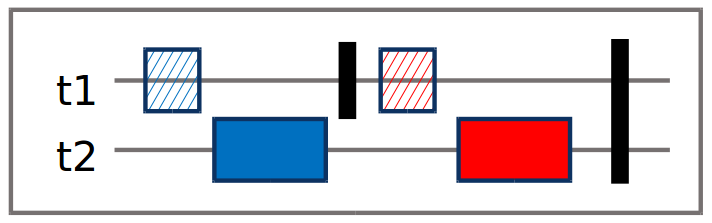
\includegraphics[width=0.48\columnwidth]{pics/intro_tasking_ex1_omp3.png}\label{fig:CodeTaskDeps3.0timeline}}
~
~
\subfloat[][]{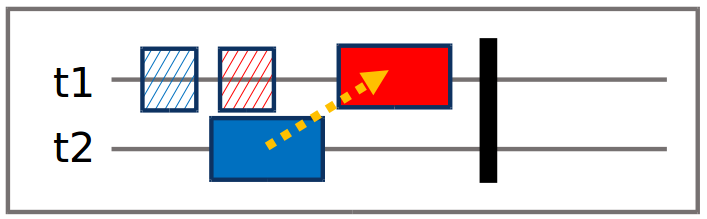
\includegraphics[width=0.48\columnwidth]{pics/intro_tasking_ex1_omp4.png}\label{fig:CodeTaskDeps4.0timeline}}
\caption{Tasking Examples without and with Dependences\label{fig:CodeTaskDeps}}
\end{figure}

The \texttt{depend} clause in OpenMP~4.0 uses variable names to indicate
dependences between tasks (i.e., restrictions on their execution order).
Figures~\ref{fig:CodeTaskDeps3.0code}~and~\ref{fig:CodeTaskDeps4.0code} show 
task code for a producer-consumer pattern in OpenMP~3.0 and~4.0.  The 
time lines below it illustrate the scheduling of the tasks on two threads.
Task dependences support fine-grained, data-driven synchronization, as 
Figure~\ref{fig:CodeTaskDeps4.0timeline} shows, which allows more flexible 
scheduling compared to the coarse-grained synchronization that OpenMP~3.0
supported (Figure~\ref{fig:CodeTaskDeps3.0timeline}). 
Figure~\ref{fig:dep-speedup} compares the parallel speedup achieved on a 
48-core system. A basic task-based implementation of Cholesky edges out a 
highly optimized version using the loop construct, and using dependences 
improves performance more significantly. For Gauss-Seidel, a basic task-based 
implementation performs worse than a version based on the loop construct, 
but a version that uses task dependences provides the best performance.

\begin{figure}
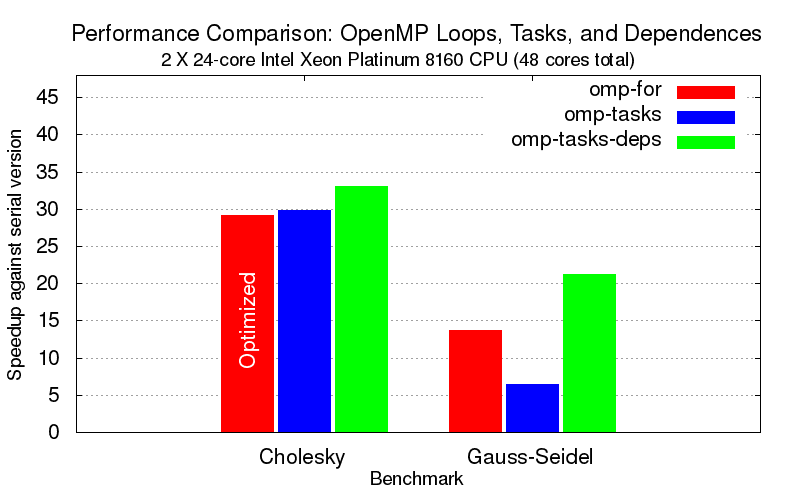
\includegraphics[width=0.45\textwidth]{pics/task-perf-results.png}
\caption{Performance Benefit of Depedendence Support}
\label{fig:dep-speedup}
\end{figure}

As stated previously, the \texttt{taskwait} construct requires that all child 
tasks of the current task must compete. The \texttt{taskgroup} construct 
allows the current task to wait on only a subset of its children, while others 
may continue executing beyond the synchronization point. Also, the construct
requires that all descendant tasks of that subset complete execution, which
we call \emph{deep synchronization}. Because some children of the current 
task can be excluded from a task group, those tasks can perform long-running 
background activities that proceed alongside successive computational kernels.

\label{sec:Taskloop}
With OpenMP~3.0 tasking support, a user could manually decompose a loop into 
chunks that OpenMP tasks execute. This cumbersome and error-prone manual 
transformation is inconsistent with the philosophy of OpenMP. Thus, OpenMP~4.5
added the \texttt{taskloop} construct to automate it. 
Figure~\ref{fig:TaskloopExample} uses the construct to parallelize a 
\emph{saxpy} operation. The \texttt{num\_tasks} clause specifies the number of 
tasks to create for the loop. Alternatively, users specify the minimum number 
of loop iterations per task with the \texttt{grainsize} clause. OpenMP~4.5
also includes a combine \texttt{taskloop simd} construct to use SIMD 
parallelism in the generated tasks.

\begin{figure}
\begin{minted}{c}
void sapxy_tasks(float * a, float * b,
                 float s, size_t n) {
#pragma omp taskloop simd             \
            num_tasks(NTASKS)         \
            shared(a,b) firstprivate(s)
  for (size_t i = 0; i < n; i++) {
    a[i] = a[i] * b[i] * s;
  }
}
\end{minted}
\caption{Task Loop Example\label{fig:TaskloopExample}}
\end{figure}
